
\documentclass[12pt,titlepage,letterpaper]{article}

\usepackage{hw}

\title{Homework II}
\author{Hanlin He (hxh160630)}
\date{\today}

\begin{document}
\maketitle

\section{MOSPF}
The multicast message would choose the route shown below.
\begin{figure}[H]
\centering
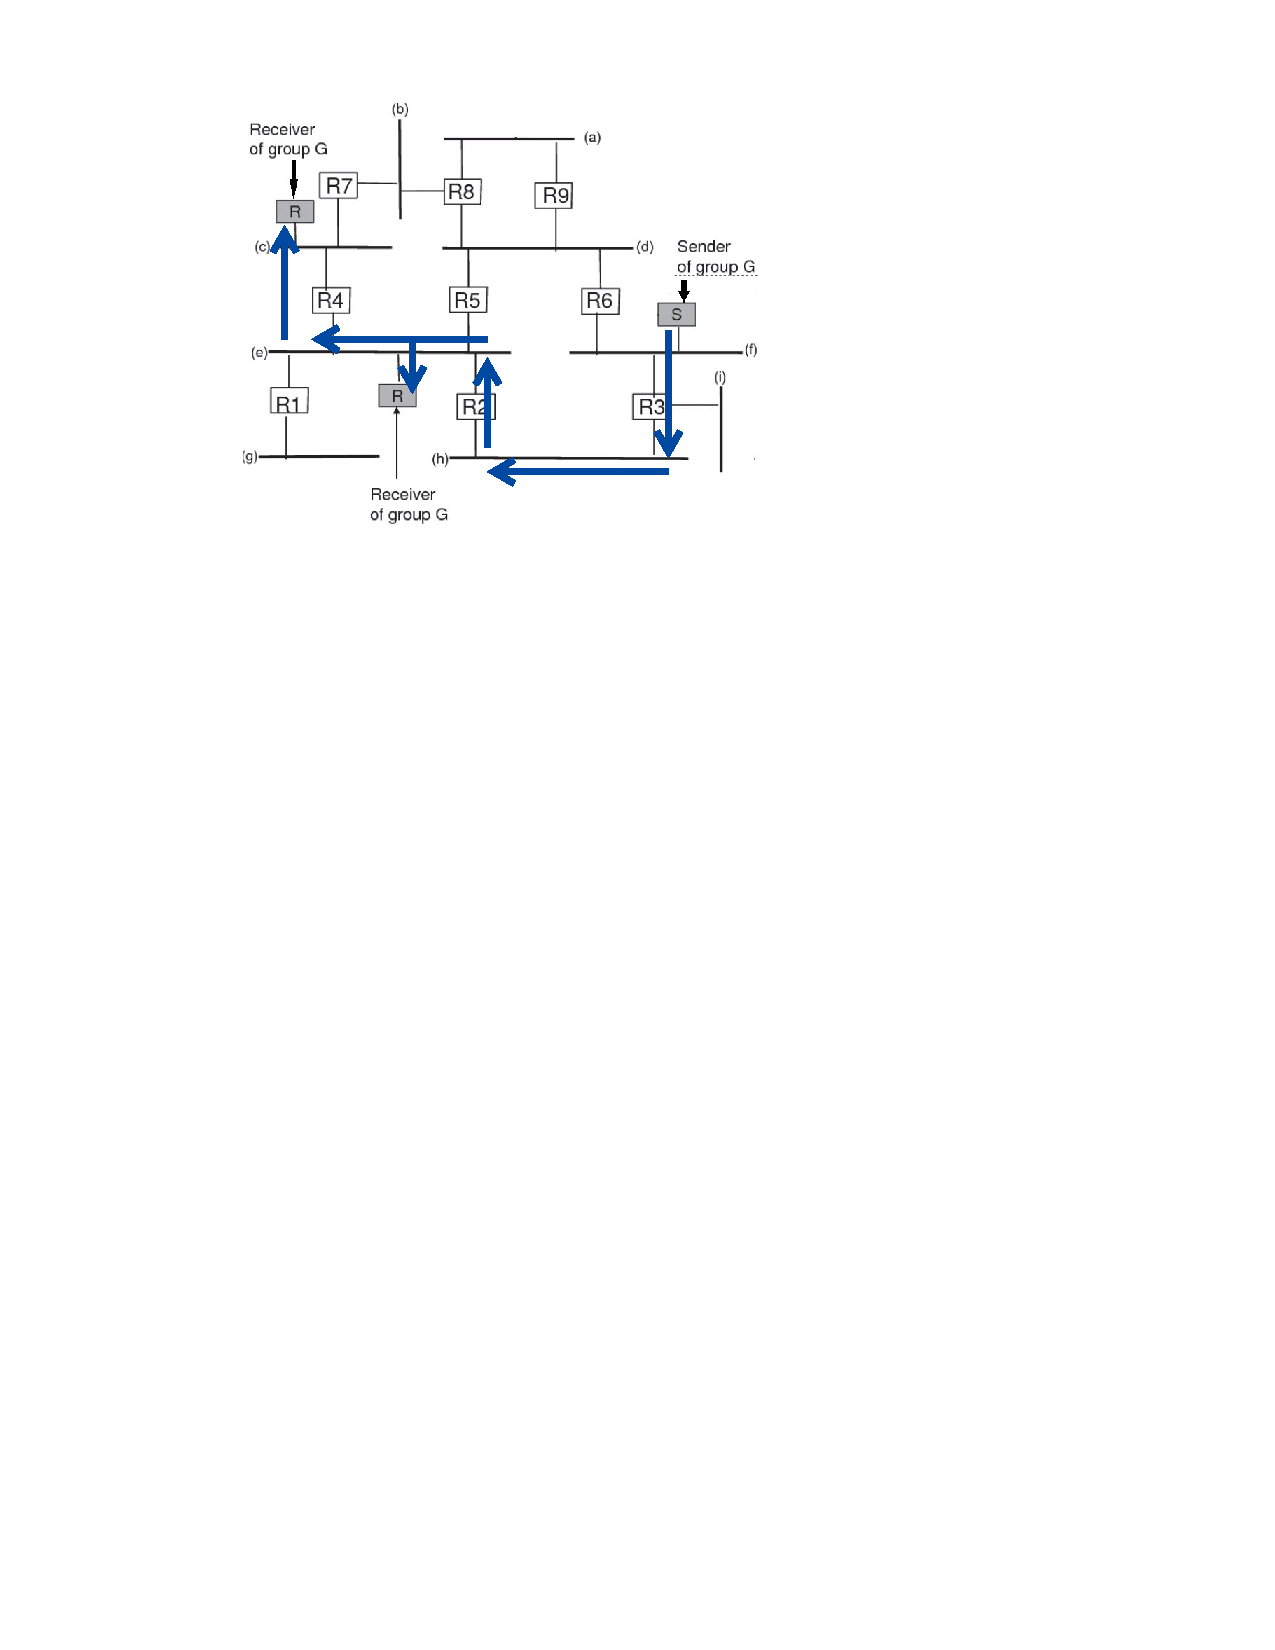
\includegraphics[width=.65\textwidth]{MOSPFd}
\end{figure}

Hence, the cache entries in each router are as follow:

\begin{table}[H]
\centering
\caption{Route Entry}
\begin{tabular}{c|c}
    \hline
    \textbf{Router} & \textbf{Cache Entry} (in format \texttt{(Ls, G, iif, MHV)}) \\\hline
    R1 & $\mathtt{(Ls, G, iif, [(e,\infty), (g,\infty)])}$ \\
    R2 & $\mathtt{(Ls, G, iif, [(e,2), (h,\infty)])}$ \\
    R3 & $\mathtt{(Ls, G, iif, [(h,2), (i,\infty), (f,\infty)])}$ \\
    R4 & $\mathtt{(Ls, G, iif, [(c,1), (e,\infty)])}$ \\
    R5 & $\mathtt{(Ls, G, iif, [(d,\infty), (e,\infty)])}$ \\
    R6 & $\mathtt{(Ls, G, iif, [(d,\infty), (f,\infty)])}$ \\
    R7 & $\mathtt{(Ls, G, iif, [(c,\infty), (b,\infty)])}$ \\
    R8 & $\mathtt{(Ls, G, iif, [(a,\infty), (b,\infty), (d,\infty)])}$ \\
    R9 & $\mathtt{(Ls, G, iif, [(a,\infty), (d,\infty)])}$ \\\hline
\end{tabular}
\end{table}

\section{PIM}

Consider four nodes \texttt{A}, \texttt{B}, \texttt{C} formed the RPT and SPT
as shown in \cref{pim}. Solid line arrow indicate the RPT from \texttt{parent}
to \texttt{child} and dashed line arrow indicate the SPT.

\begin{figure}[H]
\caption{Example}\label{pim}
\centering
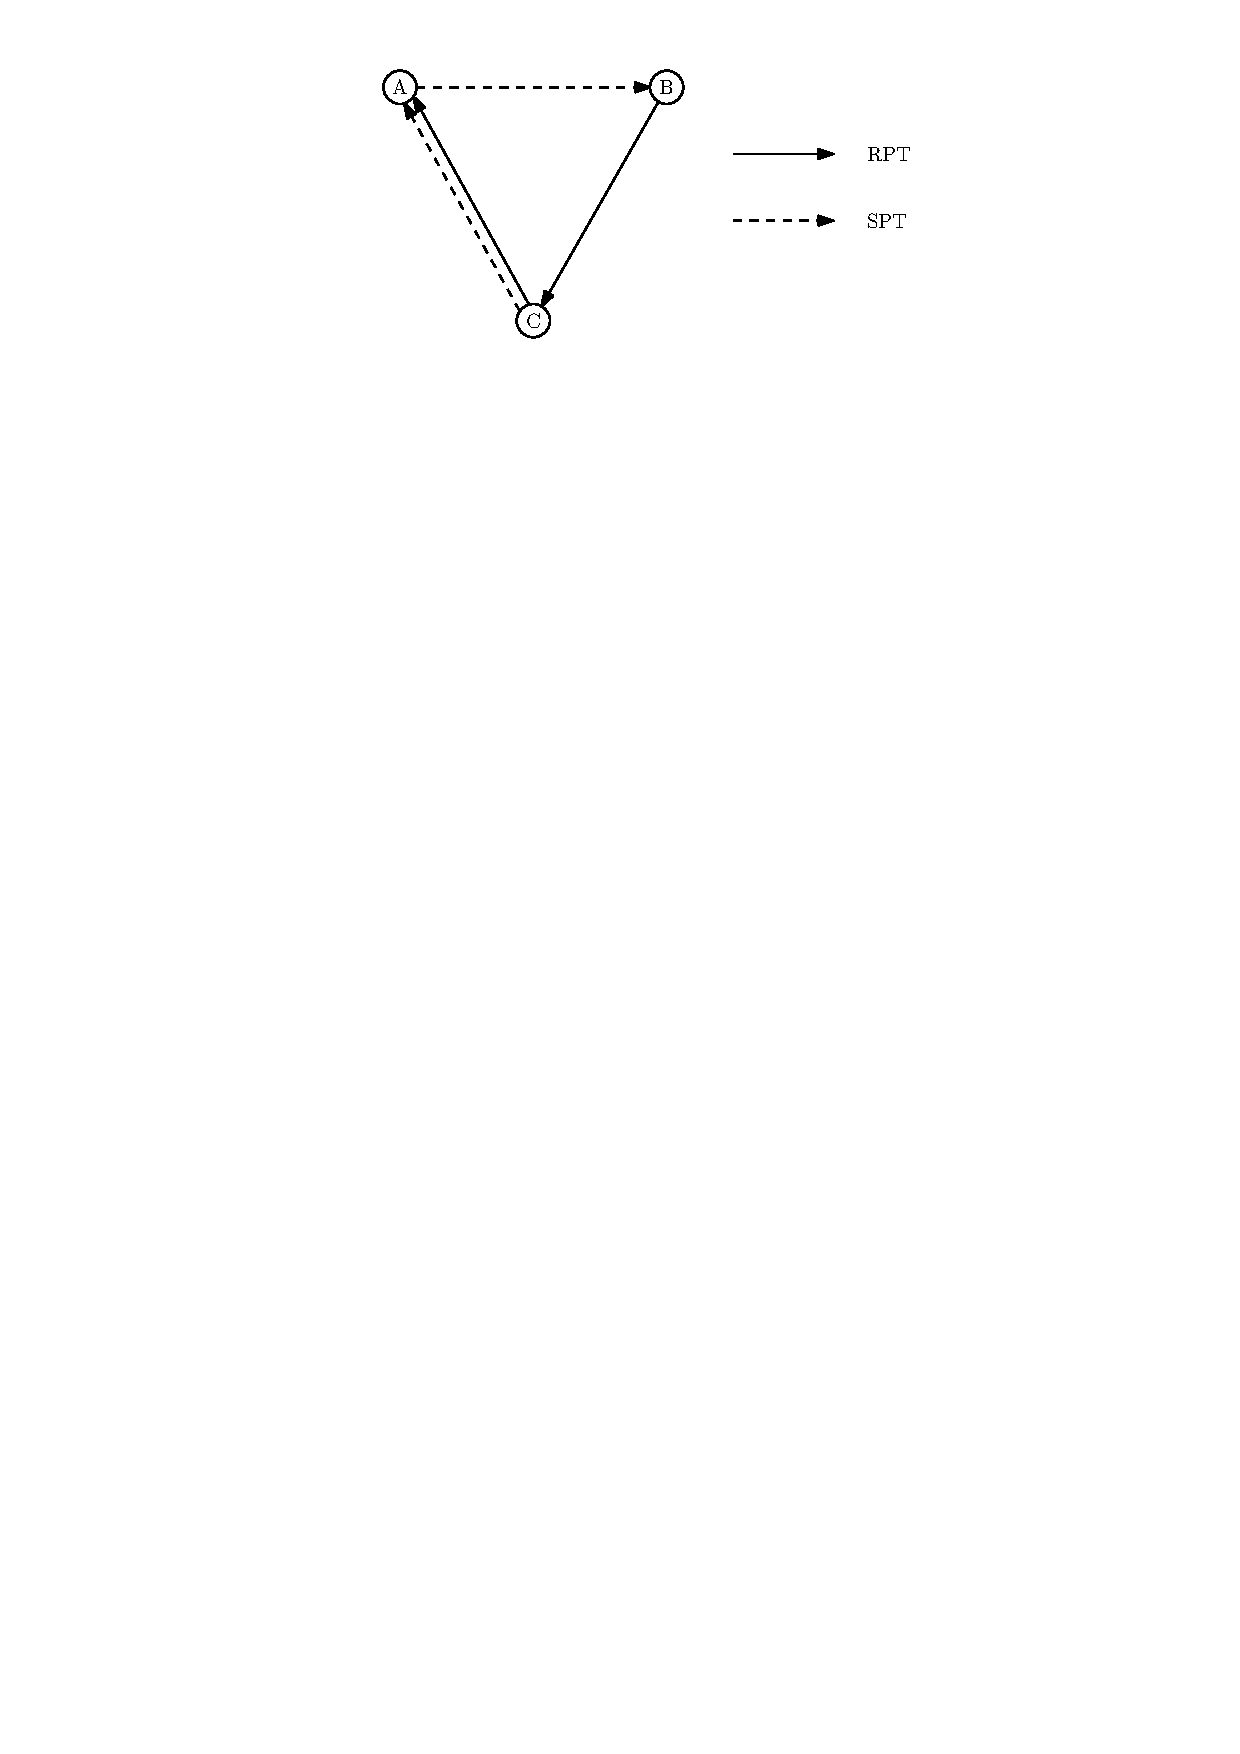
\includegraphics[width=.8\textwidth]{PIM}
\end{figure}

When node \texttt{A} received a multicast message from SPT, it would forward
the message to \texttt{B}. Since the message came from parent node in SPT,
\texttt{B} would forward the message to its child on RPT, which is \texttt{C}.
Then \texttt{C} would forward the message to \texttt{A}, since \texttt{A} is
\texttt{C}'s child on RPT.

At this point, \texttt{A} saw the multicast message for the second time.
Although the message came from the RPT parent, \texttt{C} is also the parent of
\texttt{A} on SPT. Thus, \texttt{A} could not tell which tree \texttt{C}
forward the message to. \texttt{A} would forward it anyway.

\section{PIM Inter-Domain}

In general, it will work. When join the RPT of \texttt{A}, the RP of \texttt{B}
would receive the multicast message via the RP of \texttt{A}, though some
inefficient route might exist along the RPT.

\section{OLSR}

\begin{enumerate}
    \item \textbf{Proof:}\qquad For all nodes that are $n$-hops away with a path
        of bidirectional links with source, the flood originating at source
        will reach it. We will prove the statement by induction on the hops
        number.\\
        \underline{Base Case:}\qquad For all direct neighbor nodes of the
        source, i.e., nodes that are one hop away, the flood would be directly
        received from the source. And based on MPR set definition, the MPR of
        source among all the neighbor nodes would forward the flood message to
        cover all the nodes that are two-hops away from the source.\\
        \underline{Induction Hypothesis:}\qquad Assume all node that are
        $(n-2)$-hops away with a path of bidirectional link with source
        received the flood message from source. We will prove that all nodes
        $n$-hops away will received the flood.\\
        When a node $(n-2)$-hops away received the flood. It would select it
        MPR so that the MPR set cover all nodes that are 2-hops away from it.
        Thus, the union of the MPR set of all nodes $(n-2)$-hops away would
        cover all node that are $n$-hops away. Therefore, all node $n$-hops
        away would received the flood.\\
        \underline{Conclusion:}\qquad In conclusion, all node that have path of
        bidirectional links with source would received the flood from the
        source. Hence proved if node \texttt{x} and \texttt{y} in the network,
        and a path of bidirectional links exists between \texttt{x} and
        \texttt{y}, then a flood originating at \texttt{x} will reach
        \texttt{y}.

    \item Sending the MPR set instead of MS set in TC message might work with
        some modification but would cause a much greater cost.
        \begin{itemize}
            \item Originally, only nodes which have been selected as an MPR
                would generate (and relay) TC messages. If sending the MPR set
                instead of MS set, it should be the node with non empty MPR set
                would generate the TC messages. By doing this, the topology
                based on the MPR relationship would still be complete, i.e.,
                the correct routing could be calculated.
            \item However, all nodes must have at least one MPR, otherwise the
                node is isolated with other nodes. Then, the previous
                modification indicates that all node would need to generate the
                TC message, which would greatly increase the cost.
        \end{itemize}
\end{enumerate}

\section{DSR}
When a route error message was sent to source, all intermediate nodes along the
path to source could ``eavesdrop'', and adjust cached route. But the other
nodes that are not along that path would not know. Some nodes might still use
the link from \texttt{B} to \texttt{C} to route the message. This might cause
problem if a route request arrived, the nodes might early reply with the wrong
route.

\section{Virtual Circuits}

\begin{enumerate}
    \item Because the virtual circuit ID is used to help \texttt{B} to check
        its local table more efficiently. Only \texttt{B} can decide which ID
        to use. Thus, it should be \texttt{B} to choose the virtual circuit ID
        of data from \texttt{S} to \texttt{D}.
    \item Because the virtual circuit ID is only used locally. An ID in
        \texttt{B} does not have any meaning in \texttt{A}. And there will only
        be some links at a time locally. Thus, a very small virtual circuit IDs
        is sufficient.
    \item \begin{enumerate}
        \item In setup phase, \texttt{A} informs \texttt{B} the virtual
            circuits ID associated with \texttt{p,q,r,s,t}. And \texttt{D}
            informs \texttt{C} the virtual circuits ID associated with
            \texttt{u,v,w,x,y}. \texttt{B} and \texttt{C} informs each other
            and \texttt{A}, \texttt{D} respectively that use virtual circuit id
            10 to the other side.
        \item Virtual circuit table of \texttt{A} is shown in \cref{vcta}.
            \begin{table}[H]
                \caption{Virtual Circuit Table of A}\label{vcta}\centering
                \begin{tabular}{cccc}\hline
                    Input Port & Input VID & Output Port & Output VID \\\hline
                    port to p & 5 & port to B & 10 \\
                    port to q & 11 & port to B & 10 \\
                    port to r & 20 & port to B & 10 \\
                    port to s & 7 & port to B & 10 \\
                    port to t & 19 & port to B & 10 \\\hline
                \end{tabular}
            \end{table}
        Virtual circuit table of \texttt{D} is shown in \cref{d}.
            \begin{table}[H]
                \caption{Virtual Circuit Table of D}\label{d}\centering
                \begin{tabular}{cccc}\hline
                    Input Port & Input VID & Output Port & Output VID \\\hline
                    port to u & 21 & port to C & 10 \\
                    port to v & 15 & port to C & 10 \\
                    port to w & 3 & port to C & 10 \\
                    port to x & 2 & port to C & 10 \\
                    port to y & 5 & port to C & 10 \\\hline
                \end{tabular}
            \end{table}
    \end{enumerate}
\end{enumerate}

\section{MPLS}

For some destination, \texttt{A} could compute two path each from one of
\texttt{W,X,Y,Z}. And choose one of them as primary tunnel and the other as
backup tunnel. For example the primary tunnel is \texttt{W} defined with labels
14 and Pop, and backup tunnel is \texttt{X} defined by label 17, 22 and
Pop.

When \texttt{W} failed. \texttt{A} would pushing label 17 onto packets destined
to \texttt{W}. Pushing label 17 onto packets forwards them along the backup
tunnel, thereby routing traffic around the failed linked.

\section{Fair Queuing}

\begin{enumerate}
    \item $F(p_1)$ is the \emph{fake time} when finishing transmitting packet
        \emph{i} in the fake system. Since the fake system counts the round of
        bytes , no matter how the number of links changes, total round needed
        to send the packet \emph{i} is fixed, \textbf{which is the length of
        the packet \emph{i}}. Thus, these labels do not need to be modified
        once they are assigned.
    \item $C$ is the capacity of the output channel and $B$ is the number of
        backlogged flows during the interval. Hence $C/B$ is the number of
        bytes each flows are able to send per second, i.e., the round number of
        the fake system per second.\\
        Therefore $(t_2-t_1) \times C / B$ is the total round the fake system
        would progress in time interval $[t_1, t_2]$.\\
        Hence, the virtual time of $t_2$ should be:
        \[V(t_2) = X + (t_2 - t_1) \times C / B\]
\end{enumerate}

\end{document}
